%!TEX root = ../main.tex
\subsection{Decay time acceptance}
\label{sec:b02dd:decaytimefit:acceptance}

The trigger requirements as well as some input variables to the BDT result in
a decay-time-dependent efficiency. Additionally, the \velo reconstruction
(\ie the FastVelo algorithm~\cite{Callot:2011bza}) causes a drop in decay time
acceptance for events with large decay times. In order to correctly describe
these effects the $\Bd$ lifetime is constrained to $\tau =
\SI{1.519\pm0.005}{\ps}$~\cite{PDG2014} in the nominal fit and any deviation
of the decay time distribution (summed over the tags) from a pure exponential
shape is supposed to be described by cubic splines (see
\cref{sec:dataanalysis:splines}). Knots are positioned on the rising edge at
\SI{0.8}{\ps}, approximately at the turning point at \SI{2}{\ps}, and at the
boundaries of the decay time range (\SIlist{0.25;10.25}{\ps}). The
normalisation of the splines is arbitrary and it has been decided to fix the
second to last spline coefficient to $\num{1.0}$.

On signal MC the truth information is available so the shape of the decay time
acceptance can be separated from the exponential decay. This shape is compared
with the spline method described above. As the BDTs are trained and applied
separately for the two final states and might have different effects on the
shape of the decay time acceptance these two categories are studied
individually.

\begin{figure}[htb]
\centering
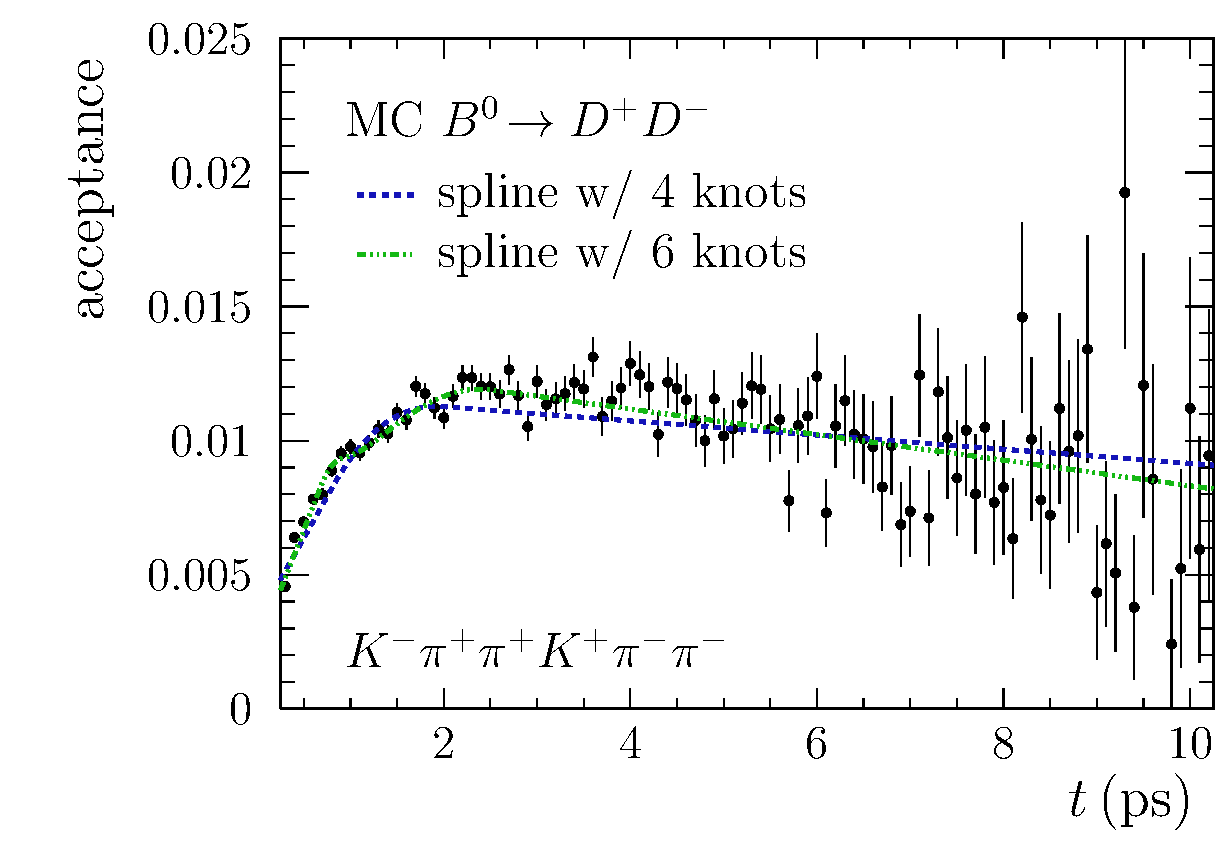
\includegraphics[width=0.48\textwidth]{07-B02DD/tikz/pdf/Acceptancespline_nolog_MC_Kpipi.pdf}
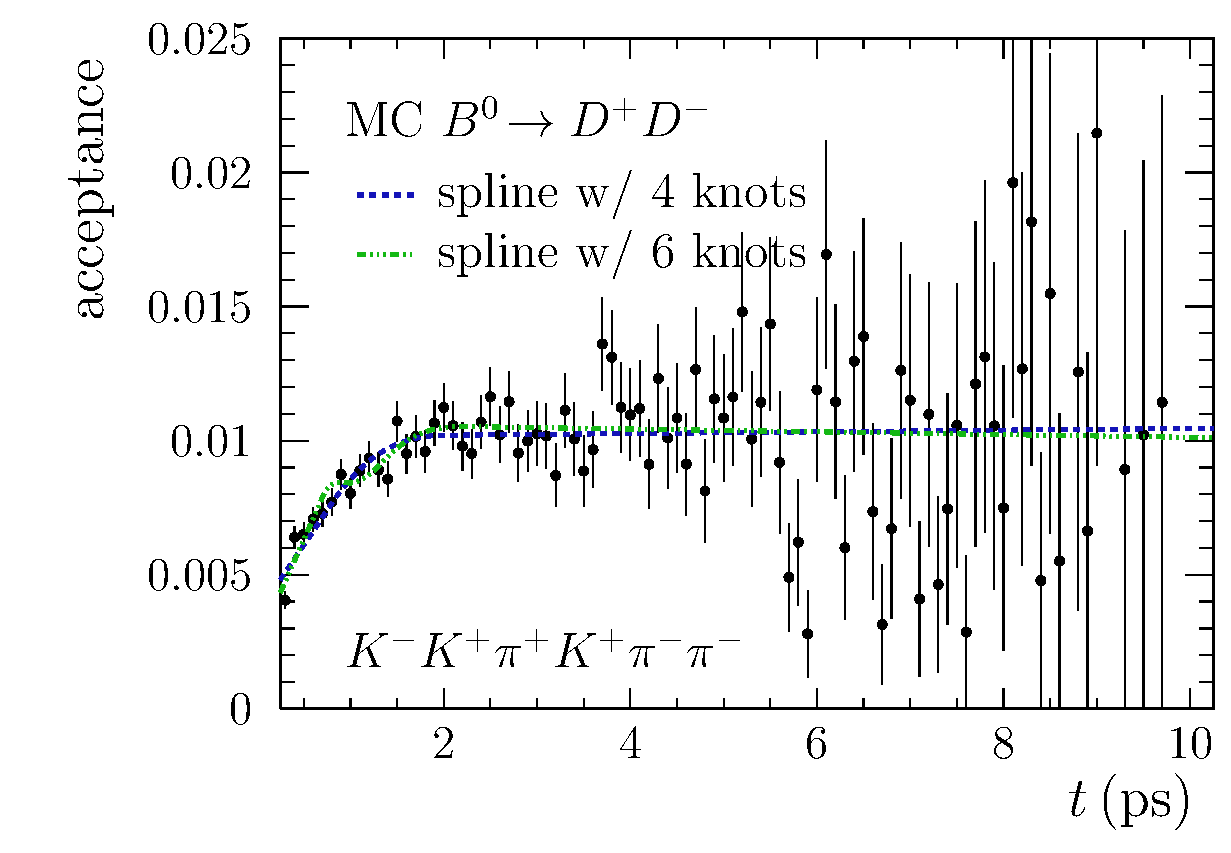
\includegraphics[width=0.48\textwidth]{07-B02DD/tikz/pdf/Acceptancespline_nolog_MC_KKpi.pdf}
\caption{Decay time acceptance of truth-matched signal MC for the $\KpipiKpipi$
final state (left) and the $\KKpiKpipi$ final state (right). The black data
points show the true decay time acceptance determined by dividing the
reconstructed by the true decay time distribution. The blue dashed line is the
spline acceptance function with four knots and the green dashed-dotted line
with six knots.}
\label{fig:b02dd:decaytimefit:acceptance_MC}
\end{figure}

Looking at the plots in \cref{fig:b02dd:decaytimefit:acceptance_MC} it is
apparent that compared to $\BdToJPsiKS$ there is a quite large efficiency loss
at high decay times. This might be related to the fact that both $\Bd$
daughter particles ($\Dp$ and $\Dm$) are relatively long-lived. The true MC
decay time acceptance is overlaid with the shape of two spline functions.
Besides the spline function with the nominal number of four knots an
additional spline function with two more knots and slightly changed positions
$(\SIlist[list-final-separator={, }]{0.25;0.7;1.0;1.5;2.5;10.25}{\ps})$ is
plotted, which gives a better description. But it has to be considered that
the statistics of the MC sample is \num{25} times larger than the real data.
Therefore, the spline function with four knots is chosen, otherwise rather
statistical fluctuations than acceptance effects would be described. The low
statistics of the $\KKpiKpipi$ final state on real data does also not allow to
use separate spline coefficients for the two final states although with the
increased MC statistics some differences become visible.
